%%==================================================
%% chapter03.tex for TJU Master Thesis
%% Encoding: UTF-8
%%==================================================

\chapter{ 代码详解}

\section{图}
\begin{lstlisting}[language=tex, label=lst:helloworld, caption=图-题注代码, numbers=left, basicstyle=\ttfamily]
\begin{figure}[!htbp]
\centering
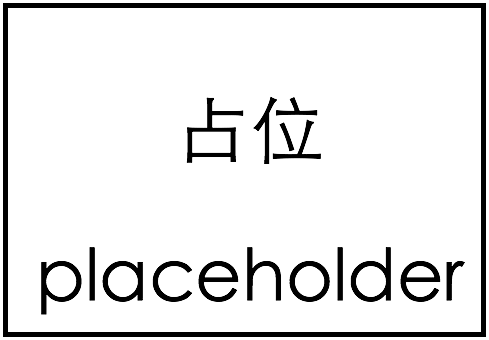
\includegraphics[width=0.5\linewidth]{figure/placeholder}
\fcaption{中文标题}{英文标题}[目录标题]
\label{fig:placeholder}
\end{figure}

\end{lstlisting}

\section{表}

\begin{lstlisting}[language=tex, label=lst:helloworld, caption=表-题注代码, numbers=left, basicstyle=\ttfamily]
\begin{table}[!htbp]
\centering
\tcaption{中文表标题}{英文表标题}[表格表标题]
\label{tab:table-example}
\begin{tabular*}{0.7\textwidth}{@{\extracolsep{\fill}}>{\hspace{0.5cm}}ccc}
\toprule
&  研究内容  &  研究方法 \\
\midrule
研究对象  &  研究内容  &  研究方法 \\
研究对象  &  研究内容  &  研究方法 \\
研究对象  &  研究内容  &  研究方法 \\
研究对象  &  研究内容  &  研究方法 \\
\bottomrule
\end{tabular*} 
\end{table}
\end{lstlisting}


